\documentclass[10pt,aspectratio=169]{beamer}

% All the boilerplate is in ccaslides.sty
% Note that this also pulls in a custom vogtwidebar.sty
\usepackage{ccaslides}

\author{Ji\v{r}\'i Lebl}

\institute[OSU]{%
Departemento pri Matematiko de Oklahoma {\^S}tata Universitato}

\title{Cultivating Complex Analysis:\\%
Line integrals (3.1 part 1)}

\date{}

\begin{document}

\begin{frame}
\titlepage
\end{frame}

\begin{frame}
A \emph{piecewise-$C^1$ path} or a \emph{path} for short
is
a continuous complex-valued piecewise continuously
differentiable function $\gamma \colon [a,b] \to \C$ 
such that $\gamma'(t)$ and all its one-sided limits are never
0.

\medskip
\pause

A path $\gamma$ is \emph{closed} if $\gamma(a)=\gamma(b)$.

\medskip
\pause

A path $\gamma$ is \emph{simple closed}
if $\gamma(a)=\gamma(b)$ and $\gamma|_{(a,b]}$ is injective.

\medskip
\pause

Piecewise-$C^1$ means that $\exists$ numbers $t_0 = a < t_1 < \cdots < t_k = b$
such that $\gamma|_{[t_{\ell-1},t_\ell]}$ is $C^1$ (up to the endpoints)
and its derivative is never zero.

\medskip
\pause

Equivalently, $\gamma$ is $C^1$ on every $(t_{\ell-1},t_\ell)$, $\gamma'$ is
never zero, and
\[
\lim_{t \uparrow t_\ell} \gamma'(t) \qquad
\lim_{t \downarrow t_\ell} \gamma'(t)
\]
exist and are never zero.

\medskip
\pause

We also consider $\gamma$ as a set, we write $\gamma$ to mean $\gamma\bigl([a,b]\bigr)$.

\medskip
\pause

E.g.,
we say $\gamma$ is in $U$ or $\gamma \subset U$ if
$\gamma\bigl([a,b]\bigr) \subset U$.
\end{frame}

\begin{frame}
\textbf{Example:}
Consider $\gamma \colon [0,4] \to \C$,

\medskip
$\displaystyle
\qquad
\gamma(t) =
\begin{cases}
t          & \text{if } t \in [0,1],\\
1 + i(t-1) & \text{if } t \in (1,2],\\
3-t + i    & \text{if } t \in (2,3],\\
i(4-t)     & \text{if } t \in (3,4].
\end{cases}
$

\vspace*{-1in}
\hspace*{2.9in}%
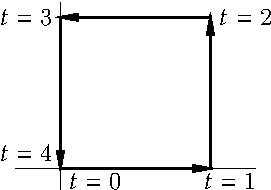
\includegraphics{../figures/squarepath}

\hspace*{0.2in}
\pause

Note, for example,
on $t \in (0,1)$, $\gamma'(t) = 1$, and so
$\lim_{t \uparrow 1} \gamma'(t) = 1$.

\medskip
\pause

Similarly
$\lim_{t \downarrow 1} \gamma'(t) = i$, etc.
\end{frame}

\begin{frame}
Given a piecewise-$C^1$ path $\gamma \colon [a,b] \to \C$ and a continuous
function $f$ on $\gamma$, 
we define the \emph{line integral} (or 
\emph{path integral}, 
\emph{curve integral},
\emph{contour integral})
\[
\int_{\gamma} f(z) \, dz
\overset{\text{def}}{=}
\int_a^b f\bigl(\gamma(t)\bigr) \gamma'(t) \, dt .
\]
\pause

The RHS makes sense:  The integrand is bounded and continuous except
at finitely many points, so Riemann integrable.

\medskip
\pause

The definition makes sense even if $\gamma'(t)$ is zero somewhere.
\end{frame}

\begin{frame}
\textbf{Example:}
Let $\gamma \colon [0,2\pi] \to \C$ given by $\gamma(t) = r e^{it}$ be
the circle of radius $r$

oriented counterclockwise: $\partial \Delta_r(0)$.

\hspace{3in}%
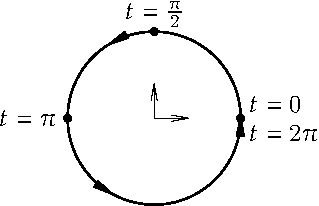
\includegraphics{../figures/circlepath}

\vspace*{-1.3in}
\pause
For $n \in \Z$, we claim

\medskip
\qquad
$\displaystyle
\int_\gamma z^n \, dz
=
\begin{cases}
2\pi i & \text{if } n=-1, \\
0 & \text{otherwise.}
\end{cases}
$

\pause
\medskip

First, $\gamma'(t) = i r e^{it}$.

\pause
\medskip

\qquad
$\displaystyle
\int_\gamma z^n \, dz
\pause
=
\int_0^{2\pi}
r^n
e^{int} i r e^{it} \, dt
\pause
=
i r^{n+1}
\int_0^{2\pi}
e^{i(n+1)t} \, dt .
$

\pause
\medskip

When $n+1=0$, the integral is $2\pi$ and $r^{n+1}=1$.

\medskip
\pause

Other $n$ are a calculus exercise.

\medskip
\pause

Note that the value of the integral does not depend on $r$.
\end{frame}

\begin{frame}
The definition is the same as the one you've seen in multivariable calculus,
\[
\int_\gamma P \, dx + Q \, dy .
\]
\medskip
\pause
Just write $dz = dx + i \, dy$, which means writing
$\gamma(t) = x(t) + i\, y(t)$:
\[
\int_{\gamma} f(z) \, dz
\pause
=
\int_{\gamma} f(z) \, (dx + i\, dy)
\pause
=
\int_{\gamma} f(z) \, dx + i f(z) \, dy
\pause
=
\int_a^b \underbrace{\Bigl( f\bigl(\gamma(t)\bigr) x'(t) + i f\bigl(\gamma(t)\bigr) y'(t) \Bigr)}_{f(\gamma(t)) \gamma'(t)} \, dt .
\]
\medskip
\pause

In fact, if you also write $d\bar{z} = dx - i \, dy$, you can write any
integral
\[
\int_{\gamma} P \, dx + Q \, dy
\qquad \text{as} \qquad
\int_{\gamma} F \, dz + G \, d\bar{z}
\]
and vice versa (exercise).
\end{frame}

\end{document}
